\documentclass[a4paper]{article}

\usepackage{amsmath}
\usepackage{amssymb}
\usepackage{parskip}
\usepackage{fullpage}
\usepackage{hyperref}
\usepackage{chronology}
\usepackage{stellar}
\usepackage{bettelini}
\usepackage{tikz}
\usepackage{fancybox}
\usepackage{array}
\usepackage{makecell}
\usepackage{booktabs}

\usetikzlibrary{cd}
\newcommand{\quotes}[1]{``#1''}

\hypersetup{
    colorlinks=true,
    linkcolor=black,
    urlcolor=blue,
    pdftitle={Geografia},
    pdfpagemode=FullScreen,
}

\title{Geografia}
\author{Paolo Bettelini}
\date{}

\begin{document}

\maketitle
\tableofcontents
\pagebreak

\part{Geografia Economica}

\section{Esercizio: la Francia ferita nell'epoca delle policrisi, Edgar Morin}

\textbf{Identifica e sintetizza in una linea del tempo i principali riferimemti storici}

\begin{chronology}[25]{1789}{2023}{\textwidth}
    \event{1789}{Rivoluzione Francese (1789)}
    \event{1830}{Rivoluzioni e crisi (1830-1906)}
    \event{1901}{Multiculturalismo francese (1901)}
    \event{1914}{Prima guerra mondiale (1901)}
    \event{1929}{Crisi economia (1929)}
    \event{1939}{Seconda guerra mondiale (1939)}
    \event{1947}{Guerra Fredda (1947)}
    \event{1956}{Crisi del comunismo (1956)}
    \event{1968}{Rivolta studentesca (1968)}
    \event{1974}{National Rally (1972)} % cambiato anno per non sovrascrivere
    \event{1989}{Caduta Muro Berlino (1989)}
    \event{2014}{Guerra Russo-Ucrania (2014)}
\end{chronology}

\textbf{Identifica i riferimenti spaziali e specifica quali sono le scale geografiche mobilitate dall'autore}

L'autore cita riferimenti spaziali su tre diverse scale geografiche.
Vengono citate per la scala nazionale nazioni con grandi influenze politiche, quali la Francia,
Russia e Stati Uniti.
Vengono citate l'Europa, Africa o l'Occidente.
Come scala più ampia viene citata quella globale.

\textbf{Definisci brevemente il termine "policrisi" spiegando l'evoluzione del concetto}

\sdefinition{Policrisi}{
    Una \textit{policrisi} è un insieme di molteplici event nefasti e interdipendenti che potrebbero
    portare a danni su grande scala (planetaria).
}

La "policrisi" sottolinea l'idea che il mondo moderno sia
caratterizzato da una profonda interconnettività.

\textbf{Proponi una riflessione argomentata sui contenuti delle ultime 4 righe del testo}

Evitare che la Francia (la Repubblica) si trasformi in uno stato del controllo
è uno degli step fondamentali per ridurre la policrisi,
essendo la Francia un importante tassello della policrisi globale.

\textbf{Riassumi in due (o tre) frasi il contenuto del testo}

Le relazioni fra eventi di scale diverse, sia a livello locale che a quello globale, 
sono interdipendenti e portano a situazioni di crisi globali.

Eventi che sono all'apparenza locali possono avere grandi effetti in crisi di scala maggiore.

\pagebreak

\section{Il secolo breve}

\sdefinition{Secolo}{
    Un \textit{secolo} può essere definito in mainera stretta come 100 anni,
    oppure come un periodo di circa 100 anni con caratteristiche omogenee.
}

Con il termine il \textbf{secolo breve} ci si riferisce al novecento.
Esso inizia con la Prima Guerra Mondiale (1914) e termina con la fine della guerra fredda.
Questa secolo è caratterizzato da una serie di avvenimenti che hanno avuto conseguenze molto importanti
per la società odienrna, in particolare le guerre mondiali.

Secondo Hobsbawm vi sono tre elementi chiave del Novecento:
\begin{itemize}
    \item la fine dell'eurocentrismo;
    \item l'unitarietà del mondo;
    \item la disintegrazione dei vecchi modelli di relazioni umane.
\end{itemize}

\subsection{Accordi Bretton Woods (1944)}

Gli \textbf{Accordi Bretton Woods} sono un accordo avente valenza economica
che porta gli Stati Uniti a ricoprire un ruolo egemone. Con questi accordigli il
dollaro assume valore. Vengono istanziati il \textbf{Fondo Monetario Internazionale},
la \textbf{Banca Mondiale} ed il \textbf{General Agreement on Tariffs and Trade}.

\sdefinition{Fondo Monetario Internazionale}{
    Il Fondo Monetario Internazionale (FMI) è un'organizzazione internazionale che mira a promuovere
    la cooperazione monetaria, la stabilità finanziaria,
    la crescita economica sostenibile, il libero scambio e la riduzione della povertà nel mondo.
    Gestisce crisi finanziarie fornendo prestiti ai paesi membri con difficoltà economiche e
    fornisce consulenza politica ed economica per favorire la stabilità economica globale.
}

\sdefinition{Banca Mondiale}{
    La Banca Mondiale è un'istituzione internazionale che mira a ridurre la povertà
    estrema e a promuovere lo sviluppo economico sostenibile nei paesi in via di sviluppo.
}

\sdefinition{GATT}{
    Il \textit{General Agreement on Tariffs and Trade} (GATT)
    è stato un accordo il quale obiettivo principale era quello di
    di promuovere il commercio internazionale riducendo le tariffe doganali,
    le discriminazioni commerciali e le restrizioni al commercio tra i paesi firmatari. 
}

Inoltre, gli Accordi di Bretton Woods sono anche connessi, ma non direttamente,
alla \textbf{World Trade Organization (WTO, 1995)}.

\subsection{Il Piano Marshall}

\sdefinition{Piano Marshall}{
    Il \textit{Piano Marshall}, ufficialmente noto come Piano di Ricostruzione Europea,
    è stato un massiccio piano di aiuti economici e finanziari offerti dagli Stati Uniti
    all'Europa occidentale dopo la Seconda Guerra Mondiale.
    Proposto dal Segretario di Stato degli Stati Uniti George Marshall nel 1947,
    questo piano mirava a sostenere la ricostruzione economica e a prevenire
    il diffondersi del comunismo offrendo assistenza finanziaria, materiale e tecnica.
}

\subsection{Crisi del 1929}

\sdefinition{Crisi del 1929}{
    La \textit{crisi del 1929} fu causata da diverse cause quali:
    \begin{itemize}
        \item speculazione eccessiva sul mercato azionario negli Stati Uniti;
        \item capacità di acquisto della popolazione minore della sovrvrapproduzione Stati Uniti;
        \item disuguaglianze economiche eccessive;
        \item prestiti delle banche sconsiderate e spesso con capitale prestato;
        \item risposta del governo degli Stati Uniti non sufficientemente rapida o efficace per affrontare la crisi.
    \end{itemize}
}

Con \textbf{Grande Depressione} si intende il periodo 1929-1939 al seguite della crisi del '29.

Questa crisi economica devastante ebbe origine negli Stati Uniti a causa del crollo del mercato azionario,
che si diffuse a livello globale.
Negli Stati Uniti, portò a una maggiore disoccupazione, povertà diffusa e un
declino drammatico dell'economia.
In Europa, la crisi portò a una serie di instabilità politiche, sociale ed economica,
facilitando l'ascesa di regimi autoritari e alimentando il malcontento sociale,
che in alcuni casi condusse a tensioni prebelliche.

La Grande Depressione rappresentò anche un elemento catalizzatore per il protezionismo economico,
con molti paesi adottando politiche di autarchia e barriere commerciali per proteggere le proprie economie,
portando a un ulteriore isolazionismo economico tra le nazioni.
Questo contesto geopolitico contribuì indirettamente allo scoppio della Seconda Guerra Mondiale.
L'instabilità economica e politica causata dalla Grande Depressione ha reso il terreno
fertile per la crescita di regimi totalitari in Europa, come il nazismo in Germania e il fascismo in Italia,
che alla fine hanno portato allo scoppio del conflitto mondiale nel 1939.

\subsection{Accordi di Jalta}

\sdefinition{Accordi di Jalta}{
    Gli \textit{Accordi di Jalta} furono un incontro tenutosi nel febbraio 1945 tra i leader delle tre principali potenze alleate della Seconda Guerra Mondiale: Stati Uniti, Regno Unito e Unione Sovietica, rappresentati rispettivamente da Franklin D. Roosevelt, Winston Churchill e Joseph Stalin.
}

Durante questa conferenza, i tre leader discussero principalmente il destino dell'Europa dopo la fine imminente della guerra. Le principali decisioni includevano:

\begin{itemize}
    \item suddivisione della Germania in quattro zone di occupazione controllate rispettivamente
        da Stati Uniti, Regno Unito, Unione Sovietica e Francia;
    \item creazione di un'organizzazione internazionale per promuovere la pace e la cooperazione tra le nazioni, che in seguito divenne l'\textit{Organizzazione delle Nazioni Unite} (ONU);
    \item i paesi liberati possono istituire liberamente i loro governi (possibilmente democratici) con elezioni libere.
\end{itemize}

\subsection{USA vs URSS}

\sdefinition{NATO}{
    La \textit{NATO} (North Atlantic Treaty Organization) è un associazione di sicurezza composta dsa diverse nazioni.
}
\begin{center}
    \begin{tikzcd}
        \fbox{\textbf{USA}}               & \textit{differenze}                       & \fbox{\textbf{URSS}}               \\
        \text{Democrazia}          & \ovalbox{\textbf{Politiche}} \arrow[r] \arrow[l]  & \text{Autocrazia}           \\
        \text{Economia di mercato} & \ovalbox{\textbf{Economiche}} \arrow[r] \arrow[l] & \text{Economia pianificata} \\
        \text{NATO}                & \ovalbox{\textbf{Militari}} \arrow[r] \arrow[l]   & \text{Patto di Varsavia}   
    \end{tikzcd}
\end{center}

% espandere commercio internazinoale
% regole vincolanti
% sistema stabile dei cambi
% 3 organi internazinoali: banca mondiale, FMI, GATT (-> WTF 1995)

\subsection{L'ascesa dell'ordine economico globale}

\sdefinition{I Trenta Gloriosi}{
    Con i \textit{trenta gloriosi} si intende quel periodo della storia (della Francia)
    che va all'incirca dal 1945 al 1975.
}

Le caratteristiche sono
\begin{itemize}
    \item Welfare state, stato sociale esteso;
    \item meno disoccupazione più posti lavoro;
    \item forte crescita econimica.
\end{itemize}

\sdefinition{Modello Fordista}{
    Il \textit{modello fordista} intrapprende l'utilizzo di tecnologie e catene di montaggio
    per la produzione lavorativa.
}

Le ragioni e le cause sono le seguenti:
\begin{itemize}
    \item Piano Marshall
    \item I nuovi accordi sul commercio mondiale
    \item La stabilità del sistema economico
    \item Progressi nella ricerca scientifica e tecnologica
    \item Imposizione / diffusione del modello fordista
    \item Disponibilità di fonti energetiche (petrolio e gas naturale) a basso prezzo
\end{itemize}

\subsection{Modello socialdemocratico}

\sdefinition{Welfare State}{
    Con \textit{Welfare State} si inende un insieme di politiche sociali
    che proteggono i cittadini dai rischi e li assistono nei bisogni circa le condizioni di vita e sociali.
}

\sdefinition{Modello socialdemocratico}{
    Il \textit{modello socialdemocratico} è un sistema politico ed economico che combina elementi del capitalismo con un forte intervento dello Stato per garantire il benessere sociale.
}

Il modello socialdemocratico è quindi un modello di Welfare State.
Le sue principali caratteristiche sono:
\begin{itemize}
    \item coerente politica estera a sostegno delle istituzioni europeiste e internazionali (come l'ONU);
    \item coinvolgimento dei sindacati e delle organizzazioni dei lavoratori nelle decisioni economiche e sociali, sostenendo la negoziazione collettiva per migliorare le condizioni lavorative;
    \item diritti civili, la libertà individuale e la partecipazione democratica, garantendo un sistema politico aperto e inclusivo.
    \item economia di mercato con un settore privato attivo, ma con un ruolo significativo dello Stato nell'economia.
        Equità fra sistema statale e privato (statalismo).
\end{itemize}

\subsection{Commercio del petrolio}

\subsubsection{Organizzazione stati esportatori di petrolio}

\sdefinition{Organizzazione dei Paesi Esportatori di Petrolio}{
    I \textit{Organizzazione dei Paesi Esportatori di Petrolio} (OPEC)
    è un'organizzazione internazionale fondata nel 1960 da alcuni paesi
    produttori di petrolio con l'obiettivo principale di coordinare e
    regolare la produzione di petrolio greggio e stabilire politiche
    comuni per influenzare il prezzo del petrolio sul mercato mondiale.
}

\subsubsection{Crisi del petrolio}

Le principali crisi del petrolio si sono verificate nel 1973 e nel 1979.

La crisi del petrolio si riferisce a diversi eventi di instabilità e aumento dei prezzi del petrolio greggio che hanno avuto un impatto significativo sull'economia mondiale. Le principali crisi del petrolio si sono verificate nel 1973 e nel 1979.

\begin{enumerate}
    \item La crisi del 1973 è stata scatenata da una serie di eventi, tra cui la guerra del Kippur tra Israele e i paesi arabi, in particolare l'OPEC, e la decisione dell'OPEC di imporre un embargo petrolifero contro gli Stati che sostenevano Israele. Questo ha portato a un repentino aumento dei prezzi del petrolio e a una grave crisi energetica, con carenze e aumenti dei prezzi dei carburanti, influenzando l'economia mondiale.
    \item La crisi del 1979 è stata causata principalmente dalla rivoluzione iraniana e dalla conseguente interruzione delle esportazioni petrolifere dall'Iran. Ciò ha ridotto l'offerta globale di petrolio e ha portato a un altro aumento dei prezzi e a ulteriori tensioni sul mercato energetico mondiale.
\end{enumerate}

Entrambe le crisi petrolifere hanno avuto impatti significativi sull'economia globale, portando a recessioni, inflazione e cambiamenti nelle politiche energetiche dei paesi, con un maggiore interesse per fonti energetiche alternative e per la diversificazione delle fonti di energia.

\subsection{I 30 gloriosi}

\sdefinition{I 30 gloriosi}{
    I \textit{30 Gloriosi} si riferiscono a un periodo di notevole prosperità economica e di crescita in Francia che va approssimativamente dal 1945 al 1975. Questo periodo è stato caratterizzato da un rapido sviluppo economico, una forte crescita industriale e un miglioramento generale delle condizioni di vita per la popolazione francese.
}

La crisi del petrolio contribuisce a terminare il periodo dei 30 gloriosi.

\subsection{I Paesi Non Allineati}

\sdefinition{I Paesi Non Allineati}{
    Con \textit{I Paesi Non Allineati} si intende una coalizione di nazoni che durante la Guerra Fredda
    si sono distinte per la loro posizione neutrale e indipendente rispetto alle potenze mondiali (USA e URSS).
}

Fondato nel 1961, il Movimento dei Paesi Non Allineati (MPNA) era composto da nazioni principalmente dell'Africa, dell'Asia e dell'America Latina, che condividevano l'obiettivo di preservare la loro sovranità nazionale, promuovere la cooperazione internazionale e difendere il diritto all'autodeterminazione.

\subsection{Fordismo e Postfordiso}

\sdefinition{Fordismo}{
    Il \textit{Fordismo} è un modello economico e produttivo sviluppato da Henry Ford,
    fondatore della Ford Motor Company, che ha rivoluzionato il settore automobilistico
    e ha avuto un impatto significativo sull'industria globale nel XX secolo.
}

Il fordismo è caratterizzato dalle seguenti proprietà:
\begin{itemize}
    \item catena di montaggio per la produzione in serie;
    \item specializzazione del lavoro;
    \item salario elevato e standardizzazione dei prodotti, riducendone i costi e permettendo ai dipendenti di acquistare i prodotti che producevano;
    \item Produce-to-Stock - si basava sulla produzione di beni in grandi quantità prima che ci fosse una domanda effettiva.
\end{itemize}

\sdefinition{Postfordismo}{
    Con \textit{Postfordismo} si intende il periodo di tempo
    successivo al declino del Fordismo, dove esso viene rivoluzionato per avere una maggiore efficienza
    sulla società ormai cambiata.
}

Le due caratteristiche sono:
\begin{itemize}
    \item flessibilità produttiva per soddisfare le esigenze velocemente;
    \item automazione tecnologica;
    \item decentramento della produzione e delocalizzazione delle fabbrice;
\end{itemize}

Il Post-Fordismo ha portato a una nuova organizzazione economica e produttiva, evidenziando la necessità di adattarsi rapidamente ai cambiamenti del mercato e incorporare innovazione e conoscenza come elementi centrali dello sviluppo economico.

\begin{table}[h]
    \centering
    \begin{tabular}{|c|c|}
    \hline
    \textbf{Fordismo} & \textbf{Post-Fordismo} \\ \hline
    Molta forza lavoro umana & Uso delle tecnologie \\ \hline
    Domanda = f(offerta), potenzialmente illimitata & Offerta o prod = f(domanda) \\ \hline
    Territorializzazione & Delocalizzazione \\\hline
    Catena di montaggio in serie & Flessibilità, just-in-time (catena di montaggio concettuale) \\\hline
    Mercati specifici, nazionali, seppur comunicanti & Mercati "transnazionali", gli Stati sono come un ostacolo \\ \hline
    \end{tabular}
    \caption{Comparison: Fordism vs. Post-Fordism}
\end{table}

\subsection{Globalizzazione}

\sdefinition{Globalizzazione}{
    La \textit{globalizzazione} è un fenomeno che coinvolge l'interconnessione e l'interdipendenza crescente tra le nazioni e le persone in tutto il mondo.
}

La globalizzazione porta su scala mondiale un incentramento di aspetti economici, sociali, culturali e politici.

I terminini \textbf{multinazionale} e \textbf{transnazionale} hanno spesso
un'accezione comune ma possono essere distinti nella seguente maniera
\begin{itemize}
    \item \textbf{Multinazionale:} si riferisce a un'azienda o un'impresa che
        ha operazioni o filiali in più di un paese.
        Queste aziende hanno una presenza globale e conducono attività in diverse nazioni,
        ma il termine non necessariamente implica che l'azienda sia completamente interconnessa
        o integrata in tutte le operazioni.
        Le multinazionali possono avere sedi in diversi paesi,
        ma le decisioni strategiche e operative possono rimanere decentralizzate.
        \item \textbf{Transnazionale:} si riferisce a un'entità o un'organizzazione che opera
        al di là dei confini nazionali.
        Questo concetto si concentra sull'idea di superare le frontiere nazionali
        e lavorare in un contesto globale,
        con un'accentuata integrazione delle operazioni e delle decisioni su scala internazionale.
        Le aziende transnazionali tendono a essere più interconnesse e
        integrate rispetto alle multinazionali e spesso cercano di operare
        in un modo che superi le limitazioni geografiche e politiche.
\end{itemize}

\subsection{Incontro Nixon 1972}

Nel 1972, il presidente degli Stati Uniti Richard Nixon compì
una storica visita in Cina, un evento che segnò un punto di svolta nelle
relazioni tra Stati Uniti e Cina e contribuì a cambiare il panorama geopolitico mondiale.

Questa visita portò ad una normalizzazione delle relazioni diplomatiche,
bilancio geopolitico (che indebolì l'URSS) e l'apertura della cina verso l'estero.

\subsection{Diplomazia del panda}

\sdefinition{Diplomazia del panda}{
    La \textit{diplomazia del panda}  una strategia utilizzata dalla Cina per sviluppare relazioni internazionali attraverso la diplomazia culturale, economica e politica, utilizzando la simpatia, la concessione di aiuti e l'uso della sua influenza economica e culturale.
}

\subsection{BRICS}

\sdefinition{BRIC}{
    I \textit{BRIC} (Brasile, Russia, India e Cina)
    sono un gruppo di nazioni povere (dagli anni 2000) con una economia
    molto promettente per l'imminente futuro, data la loro forte crescita. 
}

Dal 2010 circa i BRIC hanno un incontro informale (forum) dei capi di Stato.
I BRIC non sono quindi un ente giuridico.
Durante questo incontro viene deciso di incontrarci ogni anno, e nel 2011 viene aggiunto il Sudafrica,
facendo divenire l'accronico BRICS.

I BRICS sono caratterizzati per la loro popolosità, forte crescita economica.
Ognuno di esso ha un punto di forza specifico.
Essi vogliono presentarsi come visione/posizione alternativa all'Occidente.

\textbf{crescita eterogenea:} \\
Ad oggi il Sudafrica è il membro che ha avuto la crescita minore.
La Cina ha invece avuto invece la crescita maggiore, guadagnando il ruolo dominante.

Globalmente vi è anche una assenza di una visione comune/possibili tensioni interne.

\textbf{Brics+:} \\

\section{Polarismo}

\sdefinition{Bipolarismo}{
    Con \textit{bipolarismo} si intende contrapposizione di due blocchi distinti;
    a livello nazionale essi sono rappresentati, di solito, da due coalizioni o
    raggruppamenti di partiti e/o movimenti, che si contendono la conquista del potere. 
}

Bipolarismo e unipolarismo sono una proprietà distinta dal multilateralismo.
Il multilateralismo consiste in una cooperazione nazionale, come per esempio creare organizzazioni
come l'ONU, ma esso è indipendente dal polarismo nazionale.

Dopo la caduta del muro di Berlino, il mondo si frammenta e passa da bipolare ad unipolare.

Oltre alla poteza economica e militare (gendarme del mondo), l'America
guadagna anche un potenza sulla propria cultura, specialmente dopo la diffusione di internet
e del cinema odierna (soft power).

Prima dell'unipolarismo, lo stato autocratico con economia pianificata e
lo stato democratico conil libero mercato sono valutabili alla pari.
Dara la caduta dell'URSS, il modello Stati Uniti viene preso come apice
di modello socioeconomico.
Ciò rimane indubbio fino all'attacco dell'11 settembre 2001, dove l'attacco mette
in discussione l'aspetto culturale.
Il mondo rimane quindi unipolare fino al 2001, dove lentamente questo status si sgretola
portando ad un multipolarismo.

La presidenza Obama diminuisce la gendarmeria.

La presidenza Trump mette in pausa questo multilateralismo per mettere l'America
in primo piano a scapito degli affari esteri.
Questa presidenza aumenta anche gli interessi (export and import) con la Cina, portandone
una grande crescita economica. Questo mette in dubbio pure
il dominio economico degli Stati Uniti.

\subsection{Interpretazioni teoriche del sottosviluppo}

% TODO https://moodle.edu.ti.ch/libe/pluginfile.php/119046/mod_resource/content/1/Pass_04a_Sviluppo-A-Teorie.pdf
% Lo sviluppo di sto Rostow

Ragioni del sottosviluppo.

\begin{itemize}
    \item Una teoria del secolo scorso lega ragioni culturali al sottosviluppo (inferiorità culturale),
        ossia la cultura non permette lo sviluppo;
    \item (geo)determinismo: clima caldo, suolo arido, morfologia difficile,
        scarse risorse minerarie ed energtiche sarebbero i fattori che, secondo questa teoria, causano il sottosviluppo;
    \item Rostow: mancanza di conoscenze, infrastrutture (per produrre);
    \item Dipendenza: l'esistenza di paesi sviluppati è la causa del blocco dei paesi sottosviluppati;
    \item Integrazione: scarsa integrazione nel sistema (per raggiungere lo sviluppo per tutti basterebbe integrare tutti nel sistema).
\end{itemize}

Secondo Truman (scorso inaugurale del Presidente degli Stati Uniti d'America Harry Truman),
la causa del sottosviluppo è la mancanza di conoscenze tecniche dei popoli in questione.

Queste ragioni per il sottosviluppo sono chiaramente poco precise: ci sono
evidentemente delle situazioni dove lo sviluppo non è stato fermato dalla geografia difficile.

% testo truman 1949

% https://moodle.edu.ti.ch/libe/pluginfile.php/119047/mod_resource/content/1/ElementidiGeografia_V11.1%20156-158_2pp.pdf

\sdefinition{Visione ambientalista}{
    La \textit{visione ambientalista} o \textit{sviluppo sostenibile}
    parte dall'idea che la biosfera è un sistema
    dotato di risorse limitate e che occorra porre dei limiti allo sviluppo in
    funzione della disponibilità delle risorse. Quelle scelte in cui la differenza tra
    i tempi biologici e i tempi di produzione è tanto grande da non permettere
    la rinnovabilità delle risorse e la compatibilità con i ritmi naturali, non
    possono essere considerate sostenibili. Le relazioni tra attività umane e
    biosfera devono allora essere tali da permettere di soddisfare i bisogni e lo
    sviluppo delle culture e, nel contempo, non compromettere il contesto
    biofisico globale.
}

\sdefinition{Visione di Latouche}{
    Secondo Latouche non esistono quindi modelli universali
    ma le nozioni di sviluppo devono essere messe in relazione con la diversità
    delle culture e delle civiltà.
}

Opposte alle \textbf{visioni critiche} (visione ambientalista e visione di Latouche),
vi sono le \textbf{visioni ortodosse} (3, 4, 5).
Le visioni ortodosse hanno in comune il fatto che lo sviluppo sia direttamente legato crescita economica,
mentre le altre due indicano che lo sviluppo non è solo necessariamente legato alla crescita economia,
bensì non sono nemmeno un criterio oggettivo.

\sdefinition{Pragmatismo scientifico}{
    Il pragmatismo scientifico è una concezione nata dalla metà degli anni Ottanta.
    Essa spiega il sottosviluppo con un insime di cause esterne (la storia, situazione mondiale, azione del Nord, delle multinazionali, ecc.)
    e interne (regimi inefficienti, ecc.).
}

% https://moodle.edu.ti.ch/libe/pluginfile.php/119472/mod_resource/content/1/Latouche_Estratto_40_segg.pdf
Secondo Latouche lo sviluppo non può essere sostenibile in quanto
un pianeta finito non può accomodare uno sviluppo illimitato.

\subsection{Storia e interpretazioni del concetto di sviluppo}

\sdefinition{Indicatore}{
    Un \textit{indicatore} è un valore o elemento/aspetto, come il PIL, il salario medio etc.
}

\sdefinition{Indici}{
    Un \textit{indice} è un insieme di 2 o più valori.
}

% https://moodle.edu.ti.ch/libe/pluginfile.php/119548/mod_resource/content/1/Pass%2004c%20Sviluppo-C%2023-24_schede.pdf

\sdefinition{Prodotto Interno Lordo (PIL)}{
    Il \textit{prodotto interno lordo} (PIL) è pari alla somma dei beni e dei servizi finali
    prodotti da un paese in un dato periodo di tempo. Si dice interno perché si riferisce
    a quello che viene prodotto nel territorio del paese, sia da imprese nazionali sia
    da imprese estere. Se invece vogliamo riferirci solo a ciò che è prodotto da
    imprese nazionali, dobbiamo togliere dal pil quel che è prodotto sul territorio
    nazionale da imprese estere e aggiungere quel che è prodotto all'estero da
    imprese nazionali: abbiamo così il prodotto nazionale lordo (PNL).
}

Quando c'è una guerra o una catastrofe il PIL cresce, ma non aumenta il tenore di vita.

\sdefinition{Indice di Sviluppo Umano (ISU)}{
    L'\textit{Indice di Sviluppo Umano} si affianca al PIL e si inscrive
    nella logica della misurazione dello sviluppo umano che amplia la prospettiva
    della semplice crescita economica per definire il livello di sviluppo dei singoli
    paesi (è utilizzato con lo stesso fine anche per regioni e singole città).
    Questo indice si fonda sulla sintesi di tre diversi fattori: il PIL pro capite,
    l'alfabetizzazione e la speranza di vita.
}

\sdefinition{Happy Planet Index (HPI)}{
    L'\textit{Happy Planet Index} è una misura dell'effi cienza ambientale di una nazione,
    introdotto dalla New Economics Foundation
    (NEF) nel luglio 2006. Questo indice considera l'aspettativa di vita, la soddisfazione
    della vita soggettiva e una misura dei costi ambientali per considerare
    anche la sostenibilità globale.
    Questo indice aumenta con il benessere e la speranza di vita,
    ma diminuisce con l'impronta ecologica.
}

%% Indice di povertà normale

\sdefinition{Indice di Povertà Multidimensionale (MPI)}{
    Il MPI globale esamina le condizioni
    di deprivazione di una persona attraverso 10 indicatori relativi alla salute,
    all'istruzione e al tenore di vita e offre uno strumento per identificare chi è po-
    vero e in che misura lo è.
}

\subsection{Studio della popolazione}

% https://moodle.edu.ti.ch/libe/pluginfile.php/119548/mod_resource/content/1/Pass%2004c%20Sviluppo-C%2023-24_schede.pdf

% grafico della popolazione
% fase i -1928
% punto di flesso
% fase ii 1928-2100

\sdefinition{Tasso di natalità}{
    Con \textit{tasso di natalità}
    si intende il numero di nascite sul totale della popolazione
    (generalmente indicato in \textperthousand).
}

\sdefinition{Tasso di mortalità}{
    Con \textit{tasso di mortalità}
    si intende il numero di morti sul totale della popolazione
    (generalmente indicato in \textperthousand).
}

\sdefinition{Tasso di crescita naturale}{
    Con \textit{tasso di crescita naturale}
    si intende la differenza fra il tasso di natalità e quello di mortalità
    (generalmente indicato in \textperthousand).
}

\sdefinition{Tasso di fecondità}{
    Con \textit{tasso di fecondità}
    si intende il numero medio di figli per donna.
}

\pagebreak

\subsection{La transizione demografica}

Da anlisi dei dati della popolazione dei paesi industrializzati,
emerge un modello di crescita comune:
il modello della \textbf{transizione demografica}.

La transizione consiste in un calo, temporaneamente sfasato,
dei tassi di mortalità e natalità.

\begin{center}
\begin{figure}[th]
    \centering
    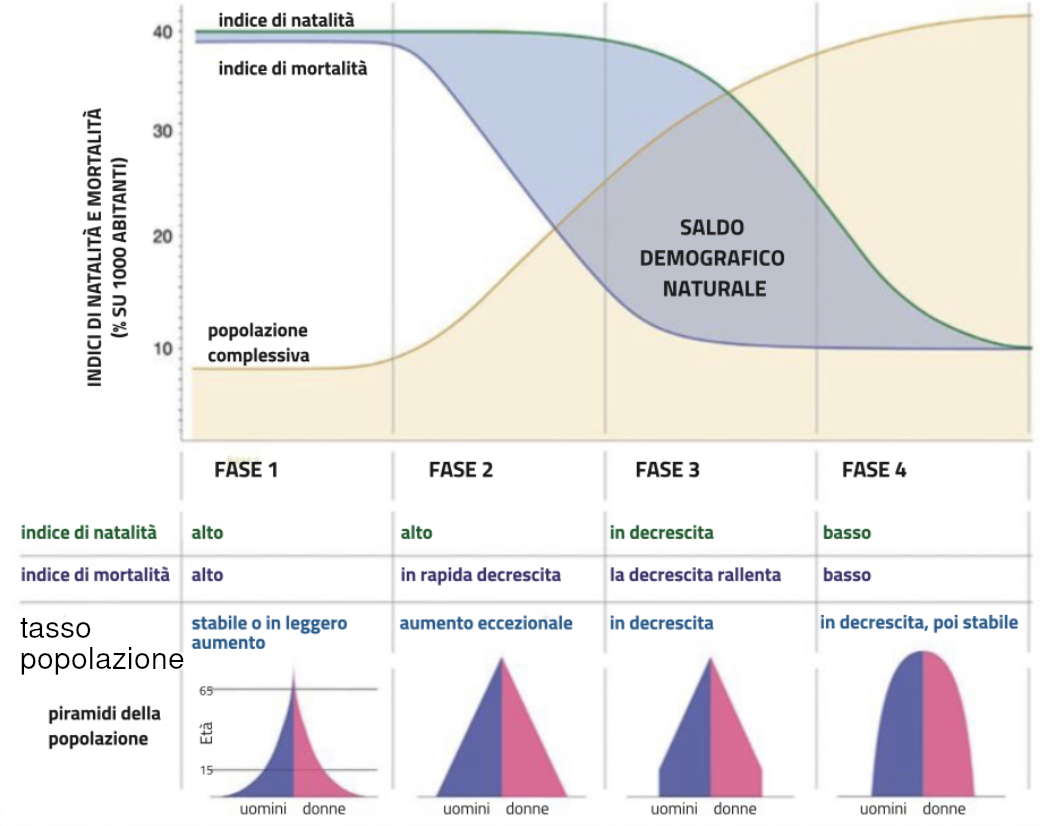
\includegraphics[width=\textwidth]{./fasi_demografia.png}
\end{figure}
\end{center}

\subsection{Migrazioni}

%% TUTTE LE COSE TIPO MIGRANTI RIFUGIATI ETC.

% migrant stocks vs flows

\newcommand{\greenbox}{
    \fcolorbox{black}{green}{\rule{0pt}{5pt}\rule{5pt}{0pt}}
}

\newcommand{\redbox}{
    \fcolorbox{black}{red}{\rule{0pt}{5pt}\rule{5pt}{0pt}}
}

Le conseguenze sociali e culturali delle migrazioni
possono essere sia positivhe che negative, sia per quanto
riguarda i paesi di partenza che, sia per i paesi di arrivo.

I paesi di arrivo hanno
\begin{itemize}
    \item \greenbox più forza lavoro e diversità;
    \item \redbox più disoccupazione, difficoltà di integrazione,
    segregazinoe, discriminazione.
\end{itemize}

I paesi di partenza hanno
\begin{itemize}
    \item \greenbox rimesse finanziarie;
    \item \redbox perdita di tradizioni,
    cambiamento della struttura demografica (meno nati, più invecchiamenti),
    fuga di cervelli.
\end{itemize}

\pagebreak

\section{Reti, nodi e flussi globali - il commercio mondiale}

% definizione di istmo

\section{La nuova via della seta cinese}

\sdefinition{Via della seta}{
    La \textit{via della seta} consiste nel reticolo, che si sviluppava per circa 8 000 km,
    costituito da itinerari terrestri, marittimi e fluviali lungo i quali nell'antichità si
    erano snodati i commerci tra l'Impero cinese e l'Impero romano. 
}

\sdefinition{Nuova via della seta}{
    La \textit{nuova via della seta} è un'iniziativa strategica della Repubblica
    Popolare Cinese del 2013 per il miglioramento dei suoi collegamenti commerciali con
    i paesi nell'Eurasia. Comprende le direttrici terrestri della \quotes{zona economica della via della seta}
    e la \quotes{via della seta marittima del XXI secolo}.
}

In inglese questa iniziativa viene chiamata \textbf{Belt and Road Initiative} (BRI),
e in Cina \textbf{One Belt One Road} (OBOR).

\sexercise{Quali obiettivi (espliciti ed impliciti) persegue il progetto OBOR (One Belt One Road) / BRI (Belt and Road initiative)?}{
    Gli obiettivi del progetto sono quelli di aumentare l'influenza della Cina
    con maggiori sbocchi commerciali (prodotti industriali cinesi, acciaio, cemento etc.),
    linee energetiche, gas e petrolio, quello di ridurre il tempo di trasporto di merci
    e creare legami di dipendenza nei confronti delle altre nazioni (con i prestiti).
}

\sexercise{Quali attori potrebbero trarre più vantaggi che svantaggi da questo progetto?}{
    In primis abbiamo la Cina, i paesi congtenenti punti che vengono attraversati
    e i punti di arrivo.
}

\sexercise{Quali attori potrebbero invece subire più svantaggi che vantaggi?}{
    Gli aspetti negativi si verificano piuttosto nei confronti dell'ambiente o
    dei lavoratori che vengono sfruttati.
}

\sexercise{Che rilevanza assume il progetto OBOR/BRI nel processo di globalizzazione}{
    XXX
}

\pagebreak

\section{Biocapacità}

\sdefinition{Biocapacità}{
    La \textit{biocapacità} è la produttività biologica di una superficie. È
    l'insieme dei servizi ecologici erogati dagli ecosistemi locali, stimata
    attraverso la quantificazione della superficie dei terreni
    ecologicamente produttivi che sono presenti all'interno della regione
    in esame.
}

La biocapacità non dipende dalle sole condizioni naturali.
La biocapacità aumenta quando sale la produttività per unità di
superficie o si ingrandiscono le superfici produttive.

L'\textit{impronta ecologica} è una sorta di contabilità delle risorse.
\begin{itemize}
    \item Essa rileva quale parte della capacità rigenerativa
        dell'ambiente è sollecitata dall'essere umano.
    \item Il metodo converte l'intensità delle utilizzazioni e dei
        carichi esercitati sulla natura, quali la campicoltura, la
        produzione di fibre vegetali o l'assorbimento di CO 2 , in
        equivalenti di superficie necessari per produrre queste
        risorse in modo rinnovabile o per assorbire le emissioni.
    \item L'impronta ecologica esprime la totalità dei consumi, di qualunque
        genere, in superficie richiesta, chiamata ettaro globale, e mostra
        in quale misura l'utilizzazione fatta della natura supera o no la sua
        capacità di rigenerazione della biosfera (biocapacità). 
    \item In tal modo, un'utilizzazione delle risorse naturali è sostenibile
        fintanto che l'impronta ecologica non superi la biocapacità.
\end{itemize}

\sdefinition{Giorno del Superamento Terrestre}{
    Il \textit{giorno del superamento terrestre} (Earth Overshoot Day)
    indica a livello illustrativo il giorno dell'anno nel quale l'umanità
    consuma interamente le risorse prodotte dal pianeta nell'intero anno stesso. 
}

La costituzione federale imposta i principi per la pianificazione del terrotorio,
ma le leggi concrete sono delegate ai cantoni.

\pagebreak

\section{Le società transnazionali}

Le imprese multinazionali sono tra gli attori più potenti dello spazio globale. La loro
internazionalizzazione è sia la conseguenza che uno dei motori della globalizzazione. Di fronte alle loro
strategie globali e ai loro modi di lavorare transnazionali, gli Stati hanno difficoltà a introdurre un
sistema di governance che possa compensare le conseguenze sociali e ambientali delle loro attività.

% https://moodle.edu.ti.ch/libe/pluginfile.php/121154/mod_resource/content/0/Le%20multinazionali_AtlasEspaceMondial_Deepl_SoloTesto.pdf

\sdefinition{Catena produttiva}{
    La \textit{catena produttiva} (\textit{global commodity chain}) è l'insieme di relazioni e di flussi che collegnao
    fra loro le imprese e gli stabilimenti produttivi coinvolti nella 
    produzione, distribuzione e commercializzazione di un bene.
}

Le multinazionale possonoc consistere nelle seguenti realtà:
\begin{enumerate}
    \item commercio materie prime \(\rightarrow\) settore I;
    \item delocalizzazione della produzione \(\rightarrow\) settore II;
    \item gestione internale dei servizi \(\rightarrow\) settore III;
    \item gruppi complessi \(\rightarrow\) (I+II+III).
\end{enumerate}

Le multinazionali hanno dei vantaggi:
\begin{itemize}
    \item Produttivi (costo minore energia, leggi estere più deboli circa lo smaltimento e consumi);
    \item commerciali;
    \item fiscali (imposte fiscali, valori diversi della merce).
\end{itemize}

l'internazionalizzazione si è avvantaggiata
soprattutto dell'apertura del commercio tra gli Stati nell'ambito degli accordi GATT
e poi dell'OMC (Organizzazione Mondiale del Commercio),
nonché della liberalizzazione finanziaria, che ha dato luogo a una maggiore mobilità dei capitali, a
una tendenza alla diminuzione dei costi di trasporto e allo sviluppo delle tecnologie
dell'informazione e delle telecomunicazioni.

L'internazionalizzazione delle multinazionali ha certamente permesso ad alcuni Paesi del Sud di
recuperare il ritardo economico - Paesi come la Cina, il cui sviluppo si basa sulla ricezione di IDE e
sull'inserimento nel processo di globalizzazione. Ma contribuisce anche ad approfondire le
disuguaglianze interne: mettendo in competizione i lavoratori dei Paesi ricchi con quelli dei Paesi
in via di sviluppo, contribuisce ad aumentare la disoccupazione nei Paesi sviluppati, che si stanno
deindustrializzando, favorendo al contempo la comparsa di classi agiate nei Paesi del Sud. Poiché
le imprese multinazionali sono spesso in posizioni di potere rispetto agli Stati, mettono questi
ultimi in competizione tra loro per l'attrattività dei loro territori (servizi, sussidi e persino
l'allentamento delle norme fiscali, sociali e ambientali).

\sdefinition{Greenwashing}{
    Con il termine \textit{greenwashing} si indica la tecnica di
    spendere una buona parte di budget pubblicitario per pubblicizzare il fatto di essere green.
}

\pagebreak

\subsection{Altro}

NIC = Newly Industralized Countries \\% China, India, Malaysia, Thailand, the Philippines, South Africa, Turkey, Brazil, and Mexic

La dottrina Truman, età dell'oro, cortina di ferro, terzo mondo.

\pagebreak

\part{Geografia Fisica}

\section{L'interazione tra le sfere terrestri}

La terra può essere suddivisa in diverse sfere interdipendenti.

\sdefinition{Atmosfera}{
    Componente gassosa che avvolge il pianeta. L'aria è inodore e incolore ed è quasi 800 volte meno densa dell'acqua.
}

\sdefinition{Idrosfera}{
    Insieme di tutte le acque del pianeta nei diversi stati di aggregazione; comprende le acque marine e quelle continentali.
}
    
\sdefinition{Litosfera}{
    Componente solida superficiale costituita dalle rocce.
}

\sdefinition{Biosfera}{
    Componente vivente e comprende gli organismi che popolano la zona di interazione delle tre sfere precedenti.
}

% TODO Astenosfera

% https://tikzcd.yichuanshen.de/#N4Igdg9gJgpgziAXAbVABwnAlgFyxMJZARgBpiBdUkANwEMAbAVxiRAB12cYAPHYAEL44AMxgAnOgF8QU0uky58hFGQAMVWoxZtO3PsACCOALaYxkmXIXY8BIgCZSDzfWatEHLr34AZXOYS0rLyIBi2ykRqzq7aHl76-ACSUOKBlrKaMFAA5vBEoCJpJkhkIDgQSE4gAEYwYFBIAMxq1iBFECWIZRXN1HUNSAC0LW0dXU3UvYjVA42II62h40jR5ZXd-fXzo8vFpVMba3PNS4X7M4d9tdvDu+ed19PHtwv37Rdr05M3g29nH0eiC+G1mr3eK0u61WWz+EIu1WmZROCwALABOMYXH5I2HzDHUBhYMDxOAQImNagACxgdHmYCYDAYUzoWAYbEgJMyUiAA
%\begin{tikzcd}
%    & \text{Atmosfera} \arrow[rdd, bend left] \arrow[ldd, bend right] \arrow[d, bend left] &                                                                                          \\
%    & \text{Biosfera} \arrow[u, bend left] \arrow[ld, bend right] \arrow[rd, bend left]    &                                                                                          \\
%\text{Idrosfera} \arrow[rr, bend right] \arrow[ru, bend right] \arrow[ruu, bend left=49] &                                                                                      & \text{Litosfera} \arrow[ll, bend right] \arrow[lu, bend left] \arrow[luu, bend right=49]
%\end{tikzcd}

I processi che coinvologno le sfere terrestri sono di due tipi:

\sdefinition{Processo Esogeno}{
    Sono processi attivati dall'energia del Sole e avvengono sulla superficie terrestre; sono per esempio i movimento delle acquem, i passaggi di stato, il tempo atmosferi o il modellamento della superficie terrestre.
}

\sdefinition{Processo Endogeno}{
    Sono processi attivati dal calore interno della Terra; sono i processi chde portano alla formazione di catene montuose e di nuovi oceani.
}

\section{Moti convettivi}

\sdefinition{Moto convettivo}{
    I \textit{moti convettivi} sono dei lenti movimenti di materiali solidi.
}

I moti convettivi possono scendere o salire.
Quando i moti salgono e colpiscono la litosfera intaccano le placche tettoniche

\begin{center}
    \bgroup{}
    \def\arraystretch{1.25}
    \begin{tabular}{ |c|c|c|c| }
        \hline
        & \textbf{Direzione scorrimento} & \textbf{\makecell[c]{Forme morfologiche che \\ si originano}} & \textbf{Esempi luoghi} \\
        \hline
        \textbf{Margini divergenti} & Direzioni opposte & Rift Valley & Dorsale medio atlantica \\
        \hline
        \textbf{Margini convergenti} & Direzioni convergenti & \makecell[c]{Isole vulcaniche \\ fossa oceanica} & Ande, Himalaya \\
        \hline
        \textbf{Margini trasformi} & Direzioni opposte & Faglie trasformi & Fagli S. Andreas\\
        \hline
    \end{tabular}
    \egroup{}
\end{center}

I tipi possibile di margine sono
\begin{itemize}
    \item Oceanica - Oceanica
    \item Oceanica - Continentale
    \item Continentale - Continentale
\end{itemize}

% leggere pag 24+ per tutte le tipologie

\subsection{Margini divergenti}

I \textit{margini divergenti}, anche detti costruittivi, avvengono quando
la densità del mantello diminuisce in un punto quando vi è una risalita di magma.

\begin{figure}[h]
    \centering
    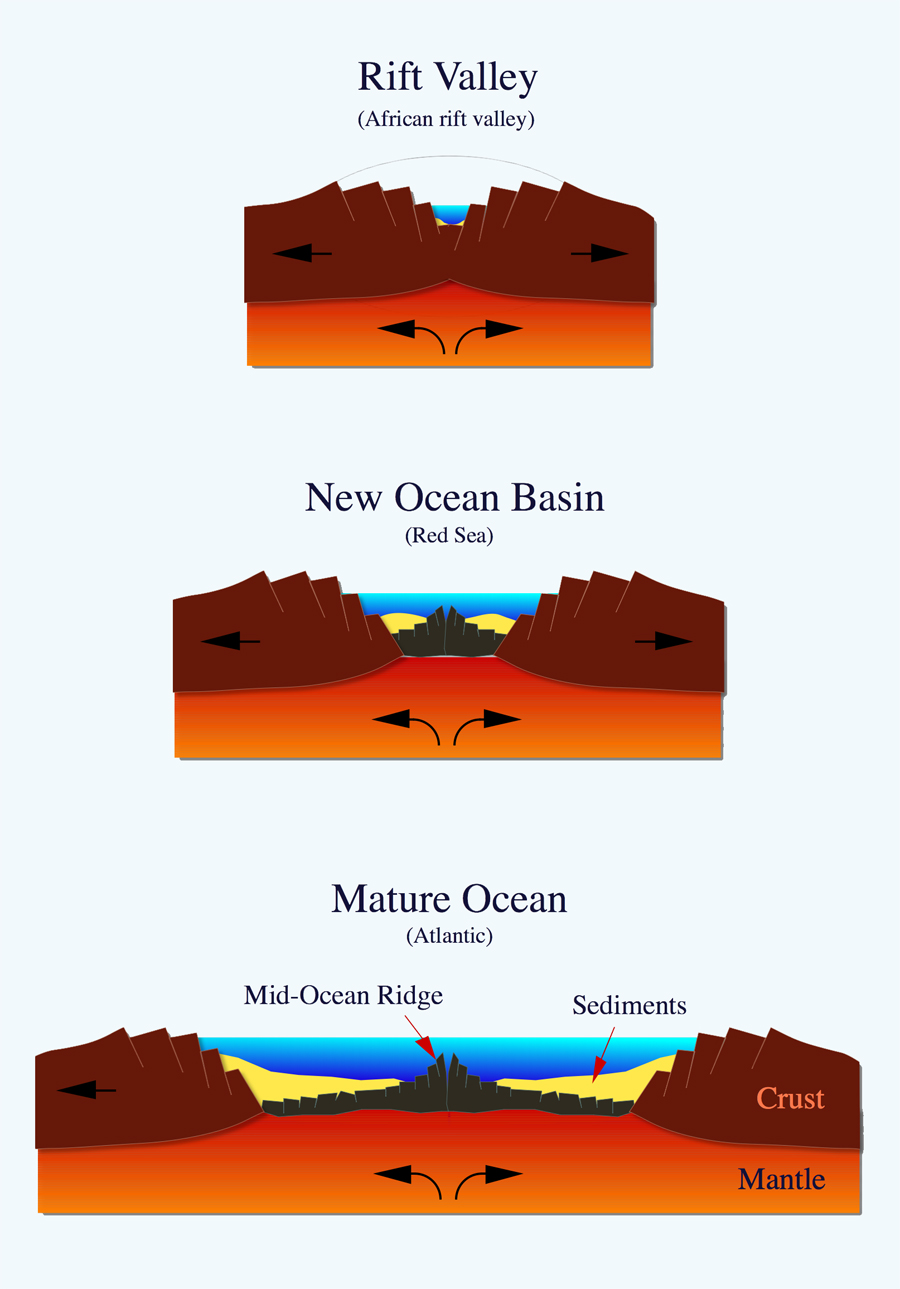
\includegraphics[width=0.5\textwidth]{rift-valley.jpg}
\end{figure}

\pagebreak

\subsection{Margini convergenti}

I \textit{margini convergenti}, anche detto di subduzione (collisione) sono distruttivi.
Essi avvengono quando due margini si scontrano.

\begin{figure}[h]
    \centering
    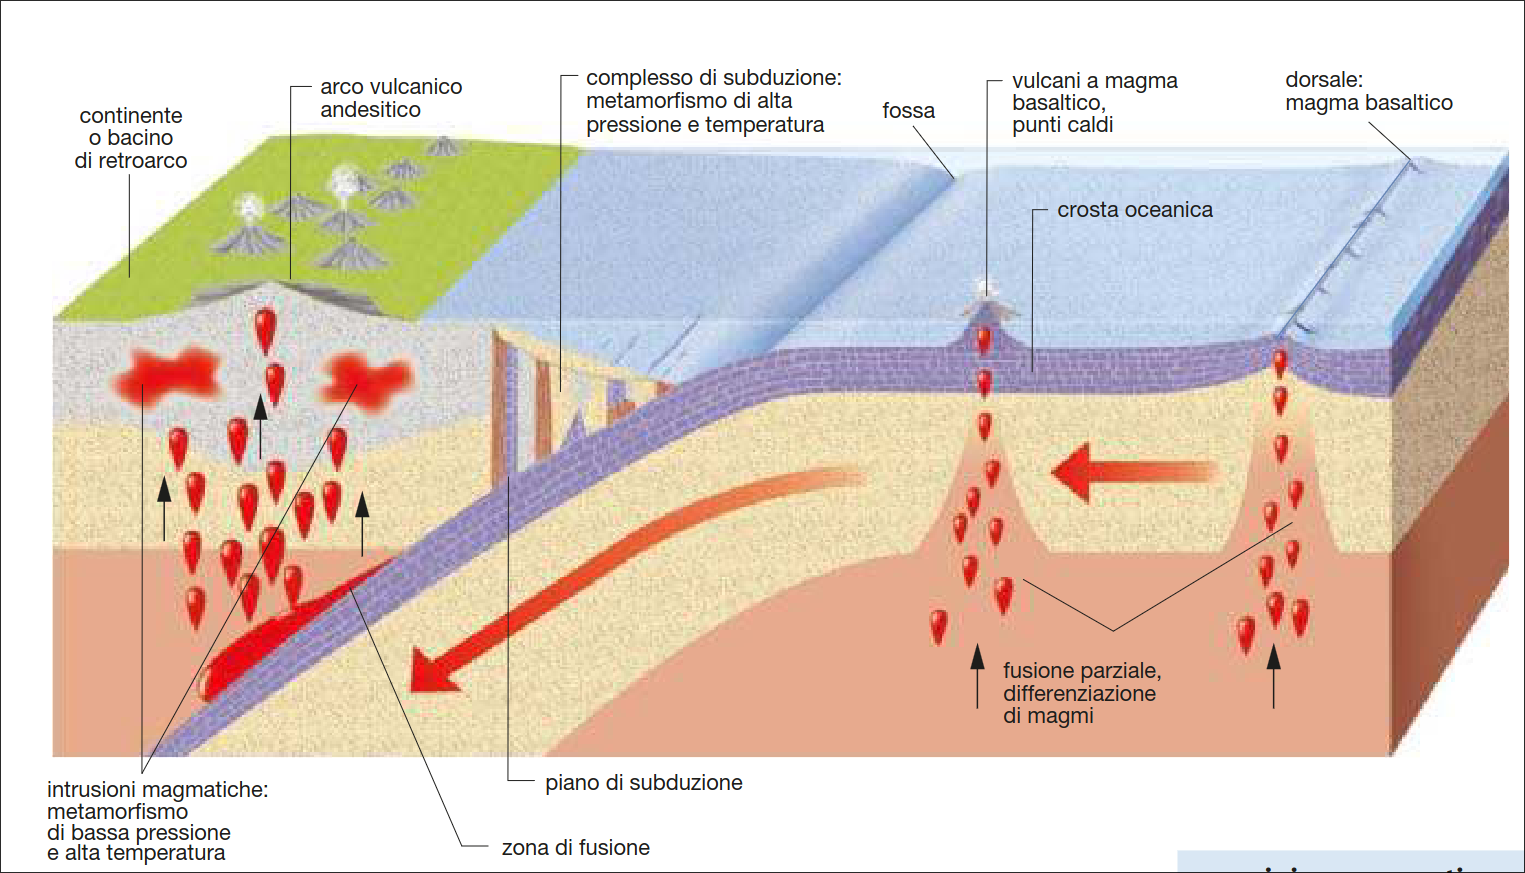
\includegraphics[width=\textwidth]{mconvergenti.png}
\end{figure}

Il materiale che fonde, risale dando origine ad attività vulcaniche.
Se i margini sono oceanica-oceanica, abbiamo una formazione di isole vulcaniche,
altrimenti si tratta di margini oceanica-continentale.

\subsection{Margini trasformi}

I \textit{margini trasformi}, anche detti conservativi e di scorrimento, avvengono quando
le placche si muovono in senso opposto a velocità differenti.
I margini trasformi non provocano vulcanismo ma violenti terremoti.

\begin{figure}[h]
    \centering
    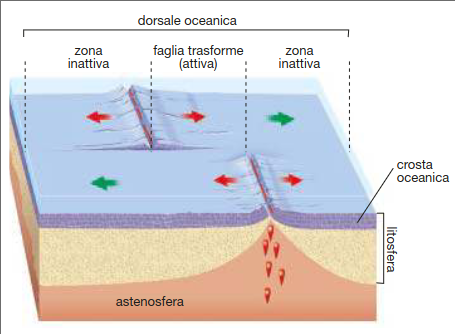
\includegraphics[width=0.65\textwidth]{mtrasformi.png}
\end{figure}

\pagebreak

\section{Terremoti}

\sdefinition{Ipocentro}{
    Con \textit{ipocentro} si indica il cuore del terremoto, in profondità.
}

\sdefinition{Epicentro}{
    Con \textit{epicentro} si indica il punto della superficie terrestre posto esattamente sopra l'ipocentro.
}

Le onde sismiche partono dall'epicentro, dove il terremoto ha generalmente un'intensità maggiore.

Vi sono onde di compressione (longitudinali) e di taglio (trasversali).
Questi due tipi di onde hanno velocità diverse, per cui il sismografo comincierà a misurarne
prima una.
Avendo molteplici sismografi è possibile localizzare l'epicentro di un terremoto.

La scala Mercalli permette di misurare l'intensità, mentre la scala Richter misura l'energia/forza di un terremoto.
Chiaramente, la scala Richter è indipendente dal punto di misurazione, mentre la scala Mercalli cambia dal punto di misurazione.

% vicino ai vulcani il terreno è più fertile.

\pagebreak

\section{Roti di rotazione e rivoluzione}

\subsection{Velocità di rotazione}

Vi sono più velocità di rotazioni: i punti su diversi cerchi di latitudine hanno diverse velocità di rotazione rispetto al centro della terra.

\sdefinition{Forza di Coriolis}{
    A causa del moto di rotazione attorno al proprio asse,
    gli oggetti che non sono ancora alle terra si spostano verso destra rispetto alla loro direzione di spostamento.
    La forza di Coriolis si applica solo alla componente dello spostamento che è perpendicolare all'equatore.
}


La forza di Coriolis è alla base della formazione dei sistemi ciclonici o anticiclonici nell'atmosfera.

\subsection{Le Stagioni}

La terra percorre un'orbita elissoidale attorno al sole. Il sole si trova in uno dei due fuori dell'ellisse.
% perielio e afelio

% TODO immagine solstizio d'estate

%L'estate avviene quando la terra è più lontana dal sole

\begin{center}
\begin{tabular}{|c|c|c|c|c|}
    \hline
    & \makecell{Solstizio \\ d'inverno} & \makecell{Equinozio di\\ primavera} & \makecell{Solstizio \\d'estate} & \makecell{Equinozio \\d'autunno} \\
    \hline
    Data & 23 dicembre & 21 marzo & 21 giugno & 23 settembre \\
    \hline
    \makecell{Parallelo in cui il sole \\ è allo Zenit (a \\ mezzogiorno)} & \makecell{Tropico del \\Capricorno} & Equatore & Tropico del Cancro & Equatore \\
    \hline
    \makecell{Luogo con il maggior \\ numero di ore di luce} & Polo Sud & \makecell{Stessa durata dì e \\ della notte su tutto \\ il pianeta} & Polo Nord & \makecell{Stessa durata del dì e\\ della notte su tutto il pianeta} \\
    \hline
    \makecell{Luogo con il minor \\ numero di ore di luce} & Polo Nord & \makecell{Stessa durata dì e \\ della notte su tutto \\ il pianeta} & Polo Sud & \makecell{Stessa durata del dì e\\ della notte su tutto il pianeta} \\
    \hline
    \makecell{Che stagione inizia \\ nell'emisfero nord} & Inverno & Primavera & Estate & Autunno \\
    \hline
    \makecell{Che stazione inizia \\ nell'emisfero sud} & Estate & Autunno & Inverno & Primavery \\
    \hline
\end{tabular}
\end{center}

\subsection{La struttura dell'atmosfera} % p. 41-43

% pagina 38 slides
Il criterio per definire lo strato dell'atmosfera è principalmente la temperatura.
L'aurora boreale si vede di notte perché è buio.

La nebbia è un fenomeno dato dalla saturazione di acqua nell'aria,
come le nuvole, il valore acque satura l'aria e crea un deposito visibile di goccioline.
Quando l'aria è satura di vapore acqueo essa si deposita su oggetti oppure piccole particelle nell'aria.

La quantità di vapore acqueo, in grammi, contenuta in un m\({}^3\) d'aria di chiama \textit{umidità assoluta}.
L'\textit{umidità relativa} è il rapporto fra quella assoluta e il valore massimo che può raggiungere.

La condensa che si forma quando apro una finestra è data dal fatto che la temperatura si abbassa, e quindi
il limite di saturazione si abbassa e l'aria diventa satura.

L'aria può salire verso l'alto per tre motivi:
\begin{enumerate}
    \item perché è calda e umida, e quindi leggera;
    \item perché incontra una montagna che la ostacola;
    \item perché si scontra con una massa d'aria più fredda ed è costretta a salirvi sopra;
    \item perché a terra, si scontra con un'altra massa d'aria ed entrambe vanno verso l'alto.
\end{enumerate}

Il vento è dato dalle differenze di pressione (come l'acqua nei bicchieri)
genera spostamenti di masse di aria.
Questa differenza di pressione è data dalla differenza di temperatura e vapore dell'aria,
la quale sale o scende creando delle correnti.
Quando l'aria si muove verso l'alto, la pressione a terra diminuisce,
mentre quando l'aria fredda scende verso il basso, la pressione a terra aumenta
(in altitudine si avrebbe l'opposto).

All'equatore (dove è più caldo), l'aria sale maggiormente, causando una pressione minore.

Il vento non scorre tuttavia dai poli all'equatore a bassa quota e dall'equatore ai poli in alta quota,
per via della forza di Coriolis.

\subsection{Circolazione planetaria}

% https://it.wikipedia.org/wiki/Modello_generale_della_circolazione
Il modello generale della circolazione divide le corrento planetarie in tre diversi fattori:
\begin{enumerate}
    \item cella polare;
    \item cella di Ferrel;
    \item cella di Hadley.
\end{enumerate}

Il fronte polare è la fascia in cui si scontrano i venti dai poli e i venti dalle medie latitudini.
Fra i due tropici è presente una \textit{zona di convergenza tropicale} data dalla bassa pressione.
Questa linea non è lineare e si sposta con la pioggia.

All'equatore piove di più perché l'aria è più calda e quindi può contenere più acqua (punto di saturazione maggiore). 

In India vi è la stagione delle pioggie. Nell'india settentrionale,
la stagione monsonica si svolge tra giugno e
ottobre, mentre nell'India meridionale la maggior parte
delle precipitazioni cade a giugno, ottobre e novembre.

\subsection{Tempo (meteorologico) e il clima}

% TODO appunti dijana

\pagebreak

\section{Cambiamento climatico}

\sdefinition{Effetto serra}{
    L'\textit{effetto serra} è un fenomeno per il quale alcuni gas
    atmosferici, detti appunti \textit{gas serra},
    permettono l'ingresso della radiazione solare proveniente dalla stella, 
    mentre ostacolano l'uscita della radiazione infrarossa riemessa dalla
    superficie del corpo celeste.
}

\begin{center}
\begin{figure}[h]
    \centering
    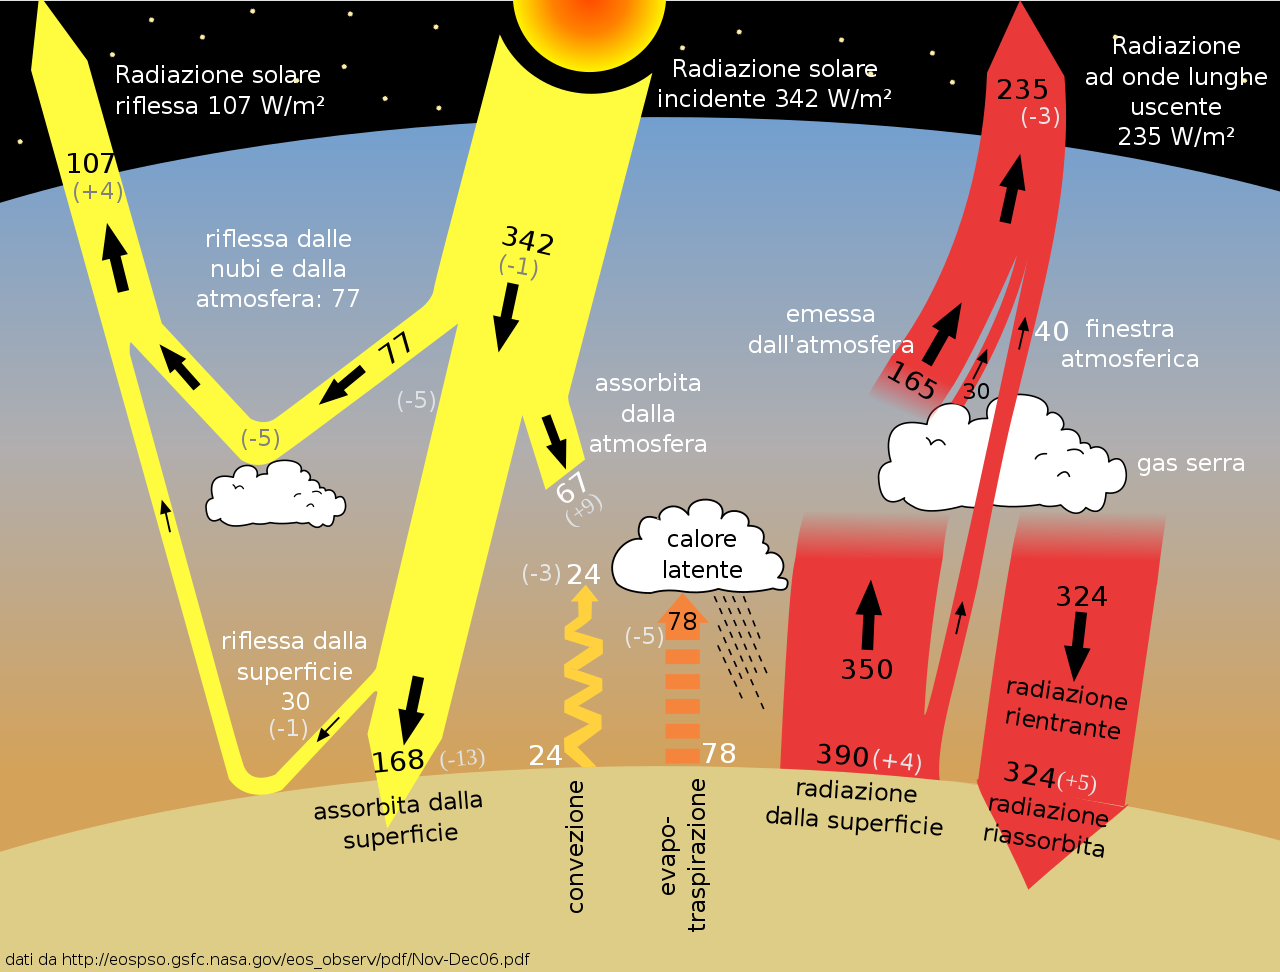
\includegraphics[width=0.75\textwidth]{./serra.svg.png}
\end{figure}
\end{center}

L'effetto serra è un fenomeno naturale, ma viene accentuato dall'essere umano.
Nessun modello riesci a rappresentare la situazione attuale senza fenomeno artificiali.
% https://it.wikipedia.org/wiki/Moti_millenari

\pagebreak

\section{Geologia della Svizzera}

\subsection{Formazione delle Alpi}

L'inizio della struttura geologica della Svizzera è dato dal formarsi delle Alpi. Tale processo
ha avuto molteplici fasi. Nel mesozoico, il medioevo geologico, la Svizzera era ancora ricoperta
dalle acque. Era parte di un esteso mare che i geologi chiamano mare di Tethys (Tetide). Sul
fondo di questo si depositò il materiale trasportato dai fiumi. Gli strati continuarono a
depositarsi uno sull'altro fino a raggiungere uno spessore valutato in varie migliaia di metri.

La formazione delle rocce sedimentarie dipendeva da vari fattori, principalmente dalla qualità
del materiale sedimentario depositato e dalle caratteristiche delle zone di mare nelle quali
queste sedimentazioni, questi consolidamenti e queste formazioni di rocce ebbero luogo. Si
distinguono essenzialmente tre zone di sedimentazione, l'area elvetica, comprendente la costa
settentrionale del Tethys, la penninica comprendente i fondali centrali, e la alpino-orientale
comprendente la costa meridionale. La crosta terrestre è suddivisa in diverse zolle, che
possono spingersi l'una verso l'altra: da ciò risulta il fatto che verso la fine del medioevo
geologico - e cioè grosso modo 100 milioni di anni fa - tutto l'insieme della terraferma situata
a sud del mare di Tethys si mise in movimento dirigendosi verso nord.
In una prima fase, e fino a enormi profondità, la zona alla deriva spinse i sedimenti depositati
in fondo al mare avanti a sé. La resistenza della massa di terraferma situata a settentrione
provocò il piegamento in falde di questi sedimenti. Prime a piegarsi furono le sedimentazioni
più molli del fondo marino situate nella zona penninica. Presumibilmente in seguito a tale
movimento il fondale marino emerse dall'acqua formando lunghe catene di isole. In un
crescendo di spinte titaniche seguì la seconda fase. A causa della pressione sempre crescente
le masse sedimentarie alpino-orientali, che inizialmente si trovavano ancora molto a sud, si
misero in moto fino a sovrapporsi alle pieghe degli strati penninici e invasero l'area di sedi
mentazione elvetica. Queste pieghe, che si protendono molto più in senso orizzontale di
quanto non si elevino verticalmente con le loro sinclinali ma che ricoprono anche superfici
caratterizzate da una massa rocciosa di diverso tipo, vengono chiamate falde di ricoprimento
o «couches». Tutta la regione alpina orientale si è formata dalla sovrapposizione di tali falde
(est-alpine). Dove questo strato di copertura, che forma un unico insieme, venne perforato in
seguito ad erosioni - per esempio nella Bassa Engadina - troviamo le cosiddette «finestre
geologiche», che portano alla luce strati penninici più profondi.
La parte occidentale e quella orientale delle Alpi si formarono in modo assai più complesso, a
causa di fenomeni geologici verificatisi nella terza fase principale della formazione delle mon
tagne. Non appena l'azione di movimenti interni determina differenze di altitudine, l'erosione
comincia a demolire le alture in formazione. Gli agenti atmosferici disgregano, decompongono
e frantumano la roccia. Le acque correnti trasportano i detriti dell'erosione. I fiumi
approfondiscono sempre più il loro alveo, erodono le montagne e producono il loro
abbassamento smantellandole.


\end{document}